\pagestyle{plain}
\chapter{PLANTEAMIENTO DEL PROBLEMA}
\section{Descripción del problema}

La construcción de edificaciones de mampostería, más específicamente de adobe, ha perdurado a lo largo del tiempo en todo el mundo dado que este recurso es abundante en el planeta. Sin embargo, los últimos acontecimientos, tal como muestra el informe periodístico realizado por \cite{France242021} sobre el terremoto ocurrido en Afganistán en el año 2021, donde se registró un terremoto de magnitud 6.3 a 35 kilómetros de la ciudad de Zindah, causando 2053 fallecidos, 9240 heridos y cuantiosas pérdidas materiales, evidencian que las viviendas existentes no estaban adecuadamente reforzadas para resistir un evento sísmico de esta magnitud.

En un estudio realizado por \cite{Ertuerk2022} en Turquía, en el distrito de Gölyaka en Düzce, se reportó un terremoto de magnitud 5.9, que causó graves daños a un total de 181 edificios de hormigón armado y mampostería. Una de las principales causas de esta vulnerabilidad fue la irregularidad en planta.

Por otra parte, en un estudio de vulnerabilidad sísmica de edificaciones realizado por \cite{Liu2023} en el distrito de Lixia, en China, se encontró que los edificios en el área urbana del distrito presentan daños leves, cumpliendo con los requisitos de fortificación sísmica. No así las edificaciones en las áreas montañosas, que presentan daños severos, mostrando que la vulnerabilidad sísmica de las edificaciones no es la misma en todo lugar.


En América Latina, \cite{Ampil2010} en un informe de la Cruz Roja Española da a conocer los datos reportados por el gobierno de Haití, en donde se narra que el 12 de enero de 2010 ocurrió un sismo de magnitud 7.3, ocasionando la pérdida de 222,570 vidas humanas, 300,572 personas resultaron heridas y las pérdidas económicas se calcularon en 7.8 billones de dólares. Todo esto fue consecuencia de la precariedad de las viviendas, siendo Haití el país más pobre del continente americano y no contando con regulaciones ni códigos antes del hecho ocurrido.

Un reporte periodístico realizado por \cite{Milo2023} de National Geographic describe el terremoto del 19 de septiembre del año 1985 como uno de los mayores desastres telúricos que sacudió al país, con una magnitud de 8.1 grados en la escala de Richter, cobrando la vida de 3,692 personas. Sin embargo, la Cruz Roja Mexicana reportó más de 10,000 muertes y cuantiosas pérdidas económicas y materiales. Este evento llevó a cambiar y rigidizar las reglas de construcción en la Ciudad de México, a tal punto que ahora solo el 4 por ciento de las viviendas son de mampostería.

En Chile, un informe técnico realizado por \cite{UGRD2010} narra el terremoto del 27 de febrero como el segundo más fuerte en la historia del país y el octavo más fuerte registrado por la humanidad, solo superado por el terremoto del año 1960. Este acontecimiento trajo consigo 525 víctimas fatales y 500,000 viviendas sufrieron daños muy graves. La mayor parte de esta tragedia la sufrieron las construcciones antiguas de su casco histórico.

En el Perú, en una nota informativa emitida por \cite{IGP2019}, se recuerda el sismo que destruyó la ciudad de Lima con una magnitud de 7.7, mostrando escenas apocalípticas de monumentos históricos caídos y edificios públicos y privados colapsados sobre sí mismos. El presidente del \ac{IGP}, el Dr. Hernando Tavera, describe que este evento sísmico cobró la vida de 252 personas, dejó 600 heridos y causó pérdidas económicas de 2,700 millones de soles. El servidor público indicó además que la fuente que incrementa la vulnerabilidad ante un sismo de estas características es la informalidad de las construcciones y la mala calidad de los materiales.

El evento trágico ocurrido en un lugar con características similares al área de estudio se evidencia en un informe del sismo redactado por \cite{INDC2014}, ocurrido el 27 de septiembre de 2014, de magnitud 5.1 en la provincia de Paruro. Como consecuencia, hubo 870 personas damnificadas, 8 fallecidos y 4 heridos, mientras que en la Comunidad de Misca se registraron 225 personas damnificadas, 45 viviendas colapsadas y 115 viviendas inhabitables.

El diario Infobae, redactado por \cite{Angulo2024}, recuerda el evento trágico del 15 de agosto de 2007, cuando un terremoto de magnitud 7.9 sacudió Pisco en Ica. El saldo del terremoto fue devastador: 596 muertos, 1,300 heridos, 76,000 viviendas destruidas e inhabitables y 432,000 damnificados. Según el informe emitido por \ac{INDECI}, luego de 275 años de silencio sísmico, sería de esperar un sismo de magnitud 8.8 próximamente, según estimaciones de \acs{IGP}. Esto nos recuerda los esfuerzos que debemos realizar en materia de prevención de desastres, como el reforzamiento de edificaciones de las familias más humildes y la concientización a través de simulacros diurnos y vespertinos.

El 28 de junio de 2024 se registró un sismo de magnitud 7 con más de 20 réplicas en Caravelí, según \cite{Leon2024}, escritora del mismo diario, teniendo como saldo 14 personas heridas y causando daños en viviendas, escuelas y centros de salud. El \ac{Ingemment} alertó sobre la existencia de 18 zonas críticas por peligros geológicos en Caravelí.

Como se puede observar en la presente investigación, la seguridad y prevención de desastres relacionados con los sismos no deberían tomarse a la ligera. El último evento sísmico registrado por el \ac{IGP} fue de magnitud 3.5, ocurrido el 24 de agosto de 2023, lo cual es un indicativo de que la región Apurímac no está exenta de este tipo de eventos, más aún cuando las autoridades del distrito de Mariscal Gamarra no realizan ningún tipo de acciones para prevenir y mitigar reduciendo la vulnerabilidad símica.

\section{Enunciado del problema}
\subsection{Problema general}
¿El diseño e implementación del reforzamiento propuesto disminuirá la vulnerabilidad sísmica en las viviendas de adobe del Centro Poblado de Paccaypata?
\subsection{Problemas específicos}
¿Cómo es la vulnerabilidad sísmica en las viviendas de adobe del Centro Poblado de Paccaypata antes de la implementación del reforzamiento estructural propuesto?

¿Cómo es la vulnerabilidad sísmica en las viviendas de adobe del Centro Poblado de Paccaypata después de la implementación del reforzamiento estructural propuesto?

\section{Justificación de la investigación} 
%  ¿Porqué elegiste este tema?
%%%%%%%%%%%%%%%%%%%%%%%%%%%%%% Justificación teórica %%%%%%%%%%%%%%%%%%%%%%%%%%%%%%%%%%%%%%%%%

La implementación de un sistema de reforzamiento económico tiene como objetivo principal disminuir la vulnerabilidad sísmica en las viviendas de adobe ubicadas en el Centro Poblado de Paccaypata. Este enfoque pretende proporcionar soluciones asequibles y efectivas que fortalezcan la estructura de las viviendas, mejorando así la seguridad de los residentes ante posibles eventos sísmicos latentes en esta región. Para fines de este estudio no se han encontrado estudios previos o parecidos en el área de estudio por lo que, realizado este trabajo de investigación se contribuirá con conocimientos valiosos sobre la solución a esta problemática.

%%%%%%%%%%%%%%%%%%%%%%%%%%%%% Justificación metodológica %%%%%%%%%%%%%%%%%%%%%%%%%%%%%%%%%%%%%%

La metodología empleada en este estudio se fundamenta en un enfoque práctico y accesible, con la finalidad de evaluar y reducir la vulnerabilidad sísmica de las viviendas de adobe en el Centro Poblado de Paccaypata mediante el diseño e implementación de técnicas de reforzamiento económico. La metodología adoptada se adapta a estas particularidades, asegurando que las soluciones propuestas sean pertinentes y efectivas en el contexto local,todo esto es crucial en un área donde los recursos económicos son escasos y el acceso a tecnologías avanzadas es limitado.

%%%%%%%%%%%%%%%%%%%%%%%%%%%%%% Justificación práctica %%%%%%%%%%%%%%%%%%%%%%%%%%%%%%%%%%%%%%%%%

La implementación de técnicas de reforzamiento económico para reducir la vulnerabilidad sísmica en viviendas de adobe en el Centro Poblado de Paccaypata se justifica de manera práctica porque el objetivo es disminuir razonablemente el riesgo de colapso durante un evento sísmico, protegiendo así la vida de los habitantes. Por otra parte tratándose de un estudio cuasi experimental, permitiría a la comunidad y otras poblaciones de características similares realizar mantenimientos periódicos sin necesidad de grandes inversiones.

\section{Ubicación y contextualización}

El área de estudio se encuentra ubicada en la región Apurímac, en la provincia de Grau,  distrito de Mariscal Gamarra. Las coordenadas geográficas del Centro Poblado de Paccaypata, según la proyección Universal Transversal Mercator (UTM), son 766164.91 metros al Este y 8472313.39 metros al Norte.

En cuanto a la accesibilidad, Paccaypata está comunicado con los distritos vecinos a través de varias vías. Al este, se conecta mediante una trocha carrozable en pésimo estado de conservación que enlaza con el distrito de Coyllurqui. Al oeste, una carretera afirmada y la más transitada, lo cual facilita la conexión con el distrito de Lambrama, permitiendo el tránsito hacia áreas vecinas y contribuye al desarrollo económico y social de la región. Hacia el norte, otra carretera proporciona acceso al distrito de Curahuasi. Al sur, una trocha carrozable conecta con la capital del distrito de Palpacachi, ofreciendo una vía adicional para el tránsito muy esporádico.
\vspace{5mm}

\begin{figure}[h!]
\captionsetup{width=\textwidth}
\centering
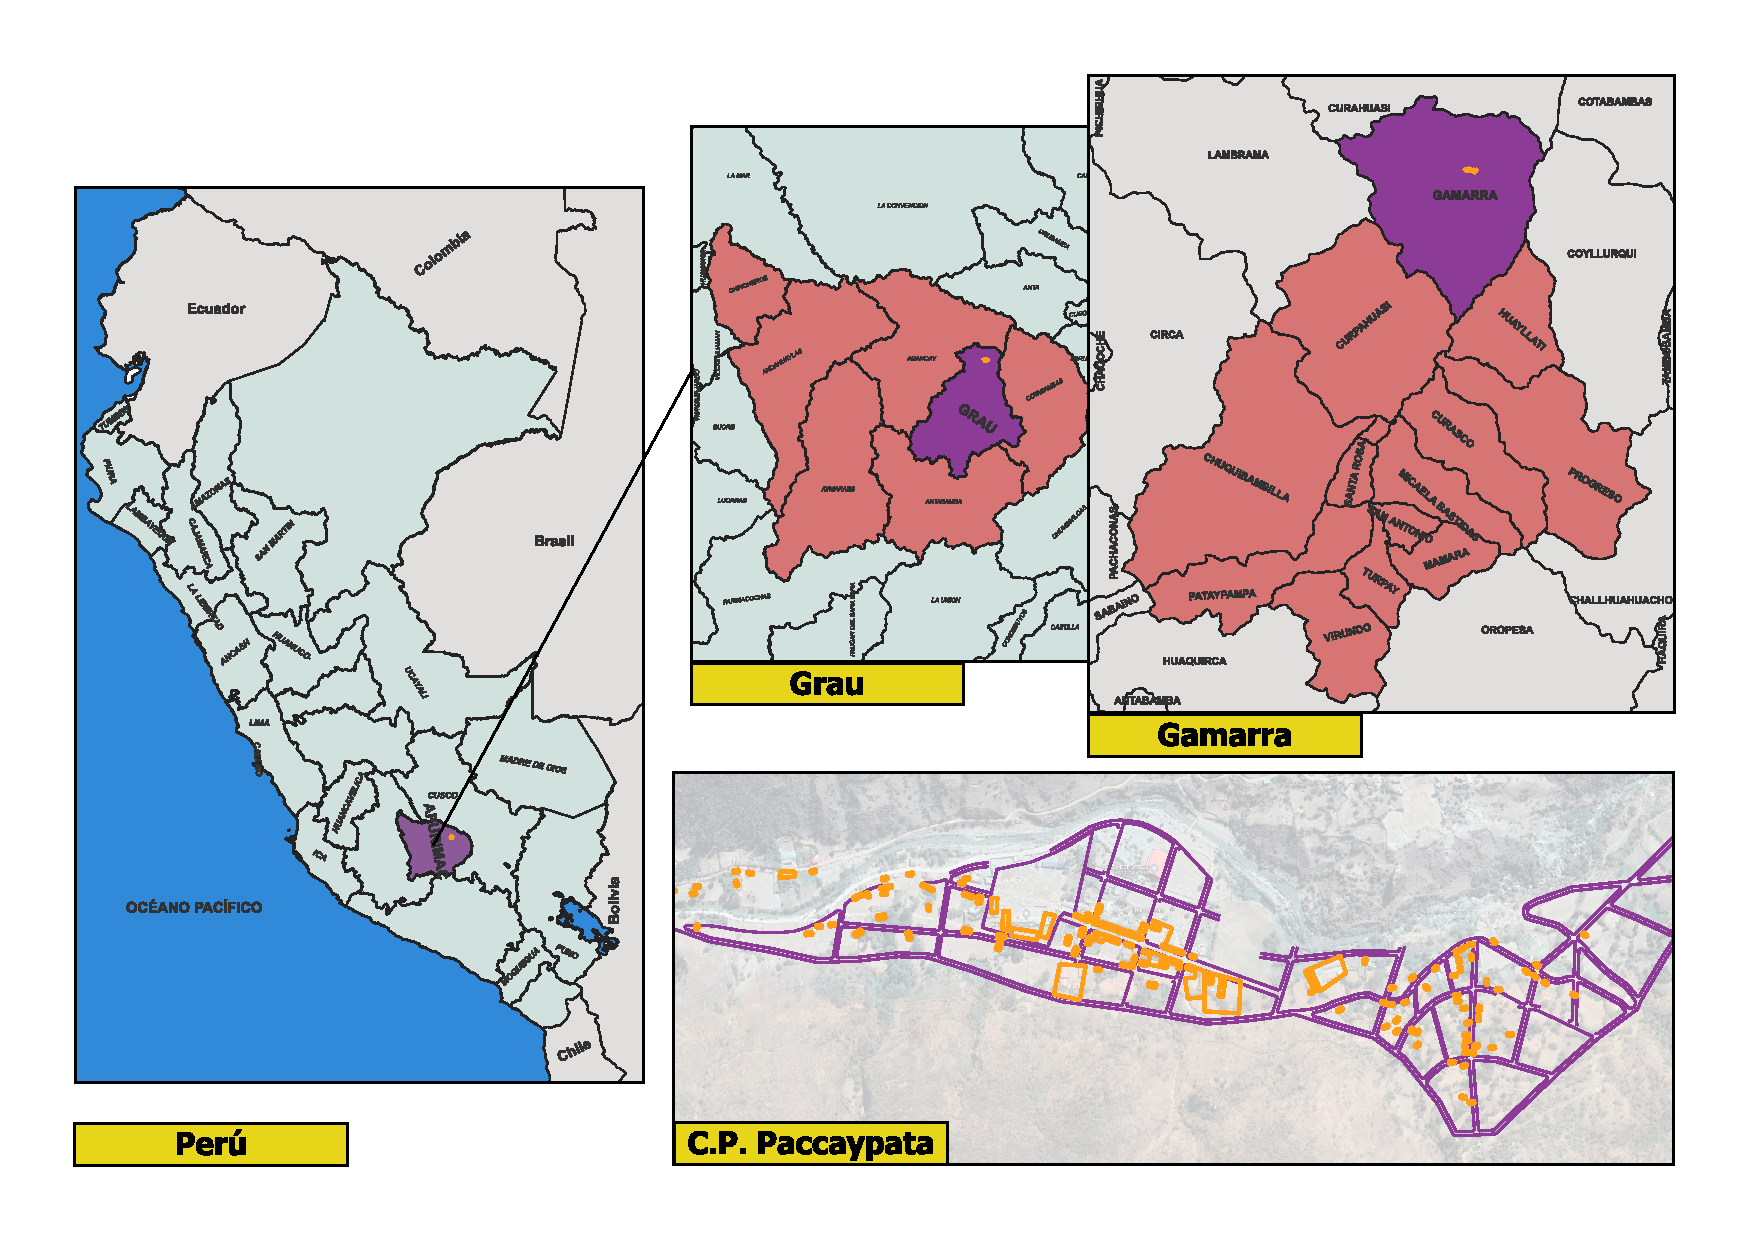
\includegraphics[width=\textwidth]{1.0.pdf}
\caption[Ubicación del Centro Poblado de Paccaypata]{El Centro Poblado de Paccaypata está ubicado en el Distrito de Mariscal Gamarra\\ Fuente: Elaboración propia}
\label{fig:1}
\end{figure}
